\documentclass[../TDO3.tex]{subfiles}%

\begin{document}
\section[s]"1"{Vidéoprojecteur}

\QR{%
	On modélise l'objectif d'un vidéoprojecteur par une lentille mince convergente
	de distance focale de \SI{5.0}{cm}. L'objet transverse a une hauteur de
	\SI{24}{mm} et l'écran se situe à \SI{4.0}{m} de la lentille. Déterminer la
	position, la nature de l'objet ainsi que la taille de l'image.
}{%
	~
	\smallbreak
	\vspace{-15pt}
	\begin{tcn}[sidebyside, sidebyside align=center](data){Données}
		\begin{enumerate}
			\item $(\ABr) = \SI{24}{mm}$~: «~l'objet transverse a une hauteur de
			      $\SI{24}{mm}$~»~;
			\item $\OAp = \SI{+4.0}{m}$~: «~l'écran se situe à $\SI{4.0}{m}$~»
			      (c'est là que se forme l'image, c'est donc la position de A')~;
			\item $\OFp = \SI{+5.0}{cm}$.
		\end{enumerate}
		\tcblower
		\begin{center}
			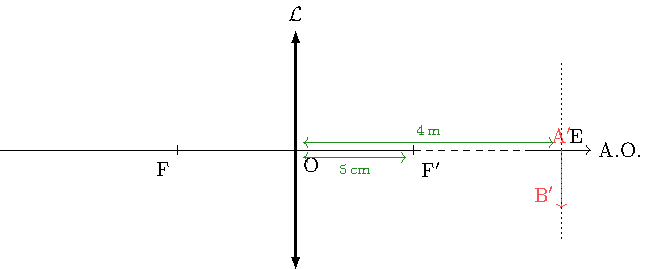
\includegraphics[width=\linewidth]{videoproj_plain}
		\end{center}
	\end{tcn}
	\begin{tcbraster}[raster columns=2, raster equal height=rows]
		\begin{tcn}(ques){Résultats attendus}
			\begin{enumerate}
				\item Que vaut $\OA$~?~: «~Déterminer la position et la nature de
				      l'objet~» (O est bon point d'intérêt à partir duquel on peut
				      mesurer des distances, et selon la valeur \xul{algébrique} de
				      $\OA$ on saura de quel côté de la lentille l'objet se situe,
				      et donc son caractère virtuel ou réel)~;
				\item Que vaut $\ABp$~?~: «~Déterminer [...] la taille de l'image~».
			\end{enumerate}
		\end{tcn}
		\begin{tcn}(tool)'r'{Outils du cours}
			\begin{enumerate}
				\item Relation de conjugaison pour une lentille mince~:
				      \[ \boxed{ \frac{1}{\OFp} = \frac{1}{\OAp} - \frac{1}{\OA}}\]
				\item Grandissement pour une lentille mince~:
				      \[\boxed{\g = \frac{\ABp}{\AB} = \frac{\OAp}{\OA}}\]
			\end{enumerate}
		\end{tcn}
	\end{tcbraster}
	\begin{tcn}[breakable, sidebyside](appl){Application}
		\begin{enumerate}
			\item De la relation de conjugaison, on a~:
			      \[
              \boxed{\OA = \frac{\OAp\OFp}{\OFp-\OAp}}
            \]
            Et avec les données,
			      \[ \xul{\OA = \SI{-5.1}{cm}}\]
			      Ainsi, on a un \xul{objet réel} situé à 5 centimètres à gauche de
			      la lentille.
		\end{enumerate}
		\tcblower
		\begin{center}
			\begin{enumerate}[start=2]
				\item De l'expression du grandissement, on a~:
				      \[\ABp = \AB\times\frac{\OAp}{\OA}\]
				      Et avec les données,
				      \[ \boxed{\ABp = \SI{- 1.9}{m}} \]
			\end{enumerate}
			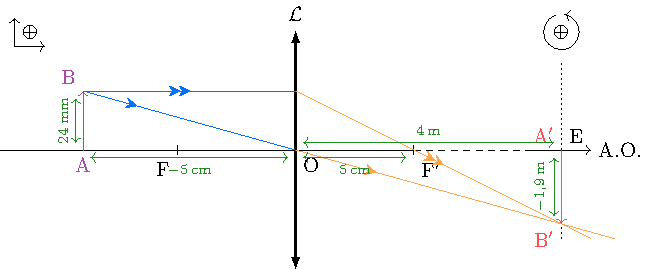
\includegraphics[width=\linewidth]{videoproj}
		\end{center}
	\end{tcn}

	\begin{tcn}(rema){Remarque}
		Attention, comme on a qu'un seul chiffre significatif, on a $\OA =
			\SI{-5}{cm}$, ce qui semble correspondre à la position de $F$, mais en
		réalité ce n'est qu'une approximation numérique. Comme $\OAp \gg \OFp$, le
		résultat numérique est proche de $-\OFp$, mais il est évident que si l'objet
		était en effet au foyer objet, le vidéoprojecteur ne formerait pas l'image
		sur l'écran mais à l'infini.
	\end{tcn}
}

\end{document}
